
\begin{center}
    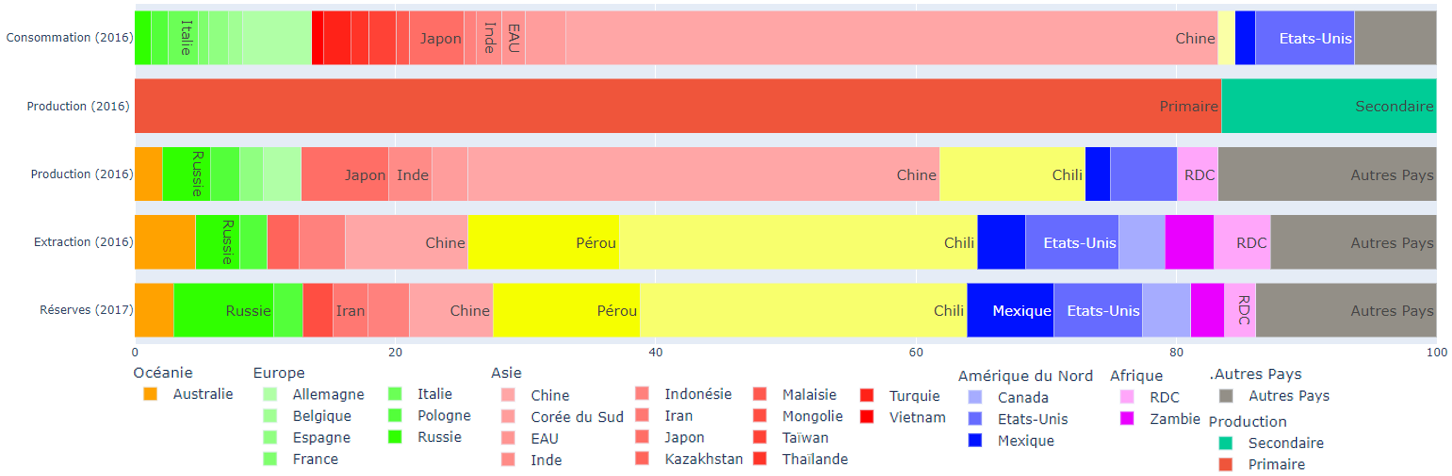
\includegraphics[width=\textwidth]{Illustration métaux/Cuivre.png}
\end{center}
\begin{center}
    \textbf{Usages et consommation}
\end{center}
La demande en cuivre est relativement corrélée au développement économique matériel global (construction, infrastrucure, équipements).
La consommation de cuivre raffiné de la Chine dépasse sa production bien qu'étant le premier pays producteur.
\begin{center}
    \textbf{Prospective}
\end{center}
\begin{multicols}{2}
    \begin{center}
        \textit{Total copper demand by sector and scenario}
    \end{center}
    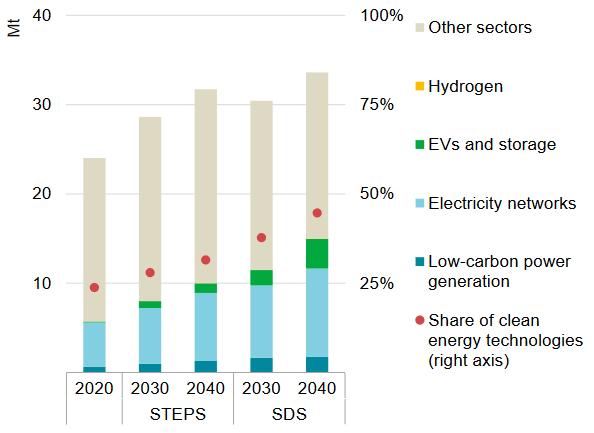
\includegraphics[width=0.45\textwidth]{Illustration métaux/Cuivre prospective.PNG}
    \vfill\null
    \columnbreak
    Il est prévu que la demande de cuivre augmente à cause du développement 
    économique mondial et de la décarbonation. Selon certains scénarios, la part de la consommation de
     cuivre pour les technologies bas-carbone
    pourrait passer de 25\% à 40\% en 2040. La demande en cuivre pour la décarbonation est
    soutenue par le développement des réseaux électriques (en particuliers distributions), 
    des véhicules électriques, des moyens de production bas-carbone.
    Les projets actuels d'extraction permettent de satisfaire la demande dans les prochaines années mais de nouveaux projets
    sont nécessaires pour satisfaire la demande à partir de 2028. La décroissance de la concentration en minerai de cuivre dans les mines
    pourrait augmenter le coût et l'impact environnemental de l'extraction.
\end{multicols}
\begin{center}
    \textbf{Production et Recyclage}
\end{center}
La production minière de cuivre a connu un taux de croissance annuel moyen de 3.25\% entre 1900 et 2016. La production minière dépasse 20 Mt/an. Cependant, les mines actuelles
sont proches de leur pic de production. La production secondaire de cuivre est passée de 2 Mt/an en 2000 à 4Mt/an en 2015.
La production secondaire a été de 42kt en 2014 pour la France sur une consommation de 248kt. La France exporte de l'ordre de 200 kt de
déchets cuivreux et en importe 50kt.
\begin{center}
    \textbf{Substituabilité}
\end{center}
Les performances électriques et thermiques du cuivre le rendent difficile à substituer. Les moteurs électriques à aimant permanent
(utilisant des terres rares) consomment moins de cuivre. Il est possible d'avoir des câbles électriques (en particulier pour les lignes aériennes)
en aluminium (moins conducteur mais plus léger).
\begin{center}
    \textbf{Prix}
\end{center}
Le prix du cuivre est assez stable. En moyenne à 6 166 US\$/t en 2017 il a atteint un pic à 10 500 US\$/t début 2022
au London Metal Exchange. La valeur de marché de la production métallurgique annuelle de cuivre est de l'ordre de 150 G US\$.

\clearpage
\begin{center}
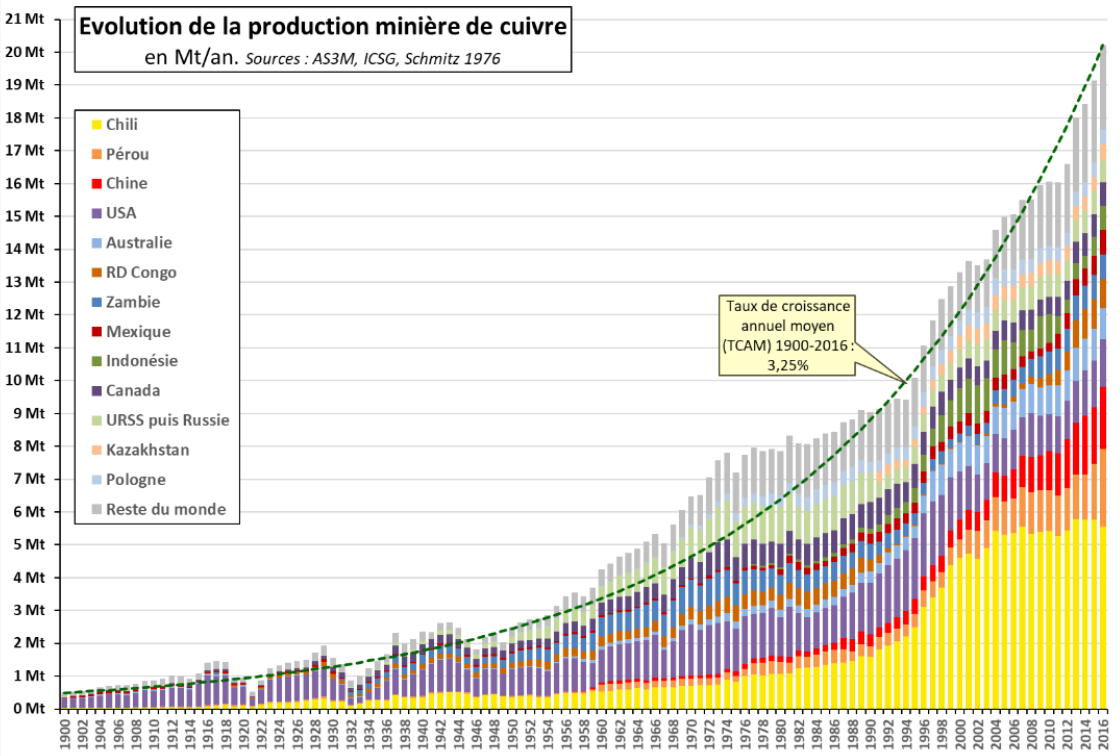
\includegraphics[width=0.7\textwidth]{Illustration métaux/Dynamique_cuivre.png}
\end{center}
\begin{center}
    \textbf{Evènements géopolitiques}
\end{center}
Il n'y a pas eu d'évènements géopolitiques notables entre 2000 et 2020.

\begin{multicols}{2}
    \begin{center}
      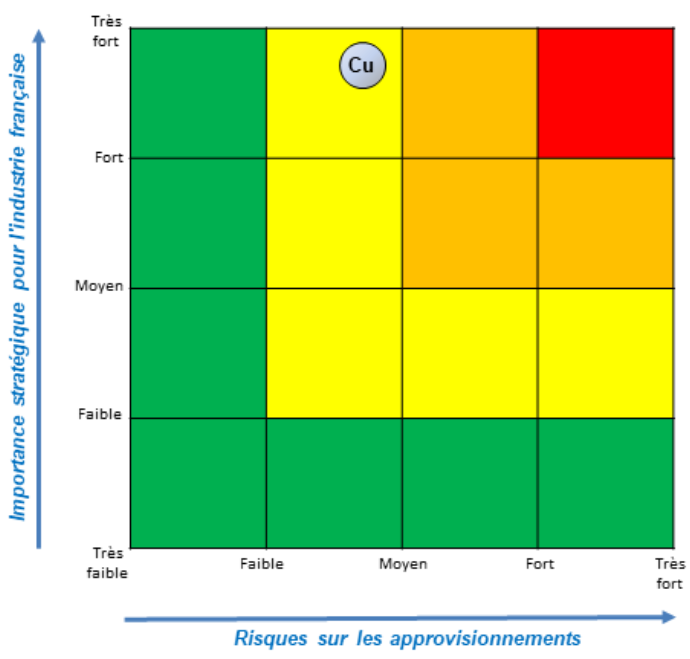
\includegraphics[width=0.35\textwidth]{Illustration métaux/Cuivre_criticité.png} 
    \end{center}
    \begin{center}
    \textbf{Criticité en France}
    \end{center}
    Le risques sur les approvisionnements en cuivre est assez faible du fait de la diversification des producteurs
    métallurgiques et miniers ainsi que de l'abondance du métal. Cependant ce métal est très fortement important pour
    la décarbonation du mix énergétique et pour l'industrie en général.
\end{multicols}

\begin{center}
\textbf{Risques spécifiques}
\end{center}
Le cuivre et le lithium sont des métaux particulièrement exposés aux stress hydriques avec la moitié de la production située dans des zones à fort stress hydrique. L'accentuation du stress hydrique par le changement climatique commence déjà à perturber l'approvisionnement par le Chili ou l'Australie.
\begin{center}
    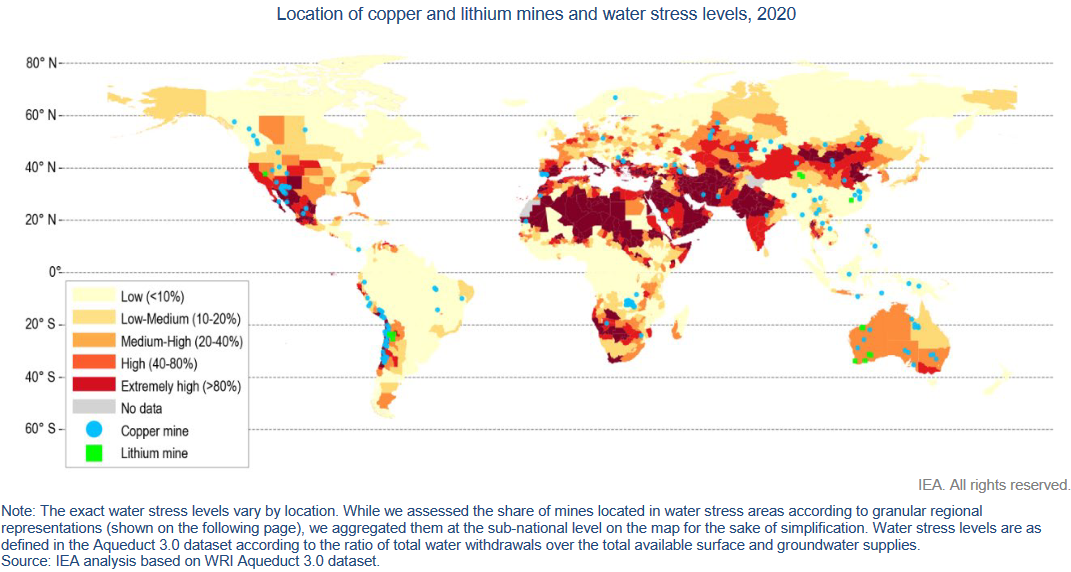
\includegraphics[width=0.75\textwidth]{Illustration métaux/risque_hydrique_cuivre.png} 
\end{center}
